
\section{Примеры движений}

Рассмотрим результаты расчетов для трех вариантов начальных условий.
\begin{enumerate}[wide]
    \item \label{sol:self_rot} Вращение вокруг своей оси ($\nu_1(0) = \nu_2(0) = 0, \nu_3(0) = 1$) (фиг.~\ref{fig:self_rot}).
    \item \label{sol:straight} Движение по прямой в направлении оси $S\xi$ ($\nu_1(0) = 1, \nu_2(0) = \nu_3(0) = 0$) (фиг.~\ref{fig:straight}).
    \item \label{sol:wrench} Движение с ненулевой скоростью центра масс и, одновременно, с ненулевой угловой скоростью платформы ($\nu_1(0) = 1, \nu_2(0) = 0, \nu_3(0) = 1$) (фиг.~\ref{fig:wrench}).
\end{enumerate}
Такие же варианты рассмотрены в \cite{GerasimovZobovaPMM2018} при интегрировании уравнений движения на гладких участках с упрощенной моделью изменения обобщенных скоростей при смене контакта.

Расчеты выполнены для симметричного трехколесного экипажа ($\alpha_i = \frac{2\pi}{N}(i - 1), N = 3$) с $n = 5$ роликами на колесе. Все величины безразмерны, так что радиусы платформы и колеса $R = 0.15$ и $r = 0.05$, массы платформы, колеса и ролика $1$, $0.15$ и $0.05$. При этом момент инерции ролика $B \approx 1.6 \cdot 10^{-5}$.
% Для безынерционной модели массо-инерционные характеристики колес положим соответствующими экипажу с пятью заблокированными роликами.

% Заметим, что снятие и наложение связей в момент контакта, вообще говоря, означает изменение системы уравнений движения. Однако в силу симметрии колеса, система после смены отличается от системы до смены лишь нумерацией роликов и углами поворота колес $\chi_i$.
% (ВАРИАНТ) % Стыковку гладких участков выполним, исходя из соображений, которые поясним на следующем примере. Рассмотрим два момента смены контакта на одном из колес: переход с ролика $1$ на ролик $2$ и переход с ролика $n - 1$ на ролик $1$. В силу симметрии колеса, система, перешедшая на второй ролик с первого, эквивалентна системе, перешедшей с ролика $n - 1$ на первый, с точностью до нумерации роликов и значений угла поворота колеса.
% Чтобы не менять вид уравнений движения -- а точнее, вид матрицы связей $\cstr$ -- выполним переобозначение в момент смены контакта и получим решение на следующем гладком участке, как решение той же системы уравнений, но с новыми начальными условиями. При смене ($\chi_i = \chi_i^+$) заменим $\chi_i = \chi_i^+$ на $\chi_i = \chi_i^-$ и циклически перенумеруем ролики. Если колесо поворачивается против часовой стрелки $\dot{\chi_i} > 0$ (см. фиг.~\ref{fig:wheel}), сдвинем индексы вперед: $j \rightarrow j+1\mod n$. Также восстановим значения обобщенных скоростей до удара $\dqdo = \cstr\nudo$, и переобозначим углы поворота роликов $\phi_{ij}$ и псевдоскорости свободных роликов после удара $\nu^+_{s(i, j)}$ соответственно выполненной перенумерации роликов. При вращении колеса в другую сторону, выполним симметричные преобразования.

Во всех трех случаях наблюдается убывание кинетической энергии скачками в моменты смены контакта. В промежутки времени между сменами энергия остается постоянной.

В вариантах \ref{sol:self_rot} и \ref{sol:straight} заметны переходные режимы вращения роликов в начале движения, когда колесо совершает первый оборот, и каждый ролик проходит полный круг, выходя из контакта и возвращаясь в него снова.

В случае \ref{sol:self_rot} вращения вокруг вертикали угловая скорость платформы $\nu_3$ в среднем медленно убывает (немонотонно): уменьшается на 5\%  за первые $10^3$с. Кинетическая энергия системы также медленно убывает. Центр масс покоится. На фиг.~\ref{fig:self_rot} приведены скорости собственного вращения роликов на первом колесе $\dot{\phi}_{1j}$. Находящийся в контакте ролик неподвижен относительно колеса (в силу связи со скоростью центра масс, см. (\ref{constraint_roller_contact}) при $\nu_1 = \nu_2 = 0$, чему соответствуют участки графиков, лежащие на оси абсцисс. Когда контакт этого ролика с опорной плоскостью прекращается, он начинает вращаться за счёт вращения экипажа в целом вокруг вертикальной оси (см. первый интеграл (\ref{int_free_roller}), существующий на гладких участках). После полного оборота колеса ролик приобретает некоторую скорость вращения, которую мгновенно теряет при следующем входе в контакт. В результате вся система теряет часть энергии, испытывая удар связями непроскальзывания. Скорость $\nu_3$ вращения экипажа вокруг вертикальной оси при этом изменяется скачком (см. например $t=1, 3, 5, 7.5$c на графиках).

При поступательном движении экипажа (вариант \ref{sol:straight}) угловая скорость тождественно равна нулю. Зависимости скорости центра масс экипажа $v = \sqrt{\nu_1^2+\nu_2^2}$ и кинетической энергии $T$ от времени показаны на фиг.~\ref{fig:straight}. Обе величины убывают (энергия -- монотонно, скачками, с каждой сменой контакта; скорость центра масс -- в среднем). Переднее колесо не вращается вокруг своей оси и движется с опорой на один и тот же ролик. Скорость вращения этого ролика связана со скоростью центра масс согласно связи (\ref{constraint_roller_contact}). Остальные ролики переднего колеса покоятся относительно экипажа. На задних колесах все ролики раскручиваются, скорости вращения показаны на фиг.~\ref{fig:straight_60_nus2}. После того как все ролики побывают в контакте, их движение становится квазипериодичным.

При комбинации поступательного и вращательного движений экипажа (случай \ref{sol:wrench}), кинетическая энергия его центра масс убывает, переходя в кинетическую энергию платформы в осях Кёнига.
Угловая скорость экипажа $\nu_3$ растет и достигает максимума (фиг.~\ref{fig:wrench_1000_nu3}) в момент $t^*_1 \approx 150$c, после чего почти монотонно убывает (с точностью до влияния первых интегралов (\ref{int_free_roller})), скорость центра $S$ экипажа $v$ становится исчезающе малой к моменту $t^*_2 \approx 300$с (фиг.~\ref{fig:wrench_1000_v}), а кинетическая энергия (фиг.~\ref{fig:wrench_1000_kin_en}) убывает при каждой смене контакта. Центр платформы $S$ описывает спираль (фиг.~\ref{fig:wrench_1000_traj}). После почти полной остановки центра масс при  $t > t^*_2$ экипаж вращается вокруг вертикальной оси $Sz$, постепенно замедляясь. Угловые скорости роликов представляют собой квазипериодические функции времени (характерный участок представлен на фиг.~\ref{fig:wrench_1000_nus1}).

\newpage

% \subsection{Вокруг своей оси}

\begin{figure}[h]
    \subf{0.3\textwidth}{
        \centering
        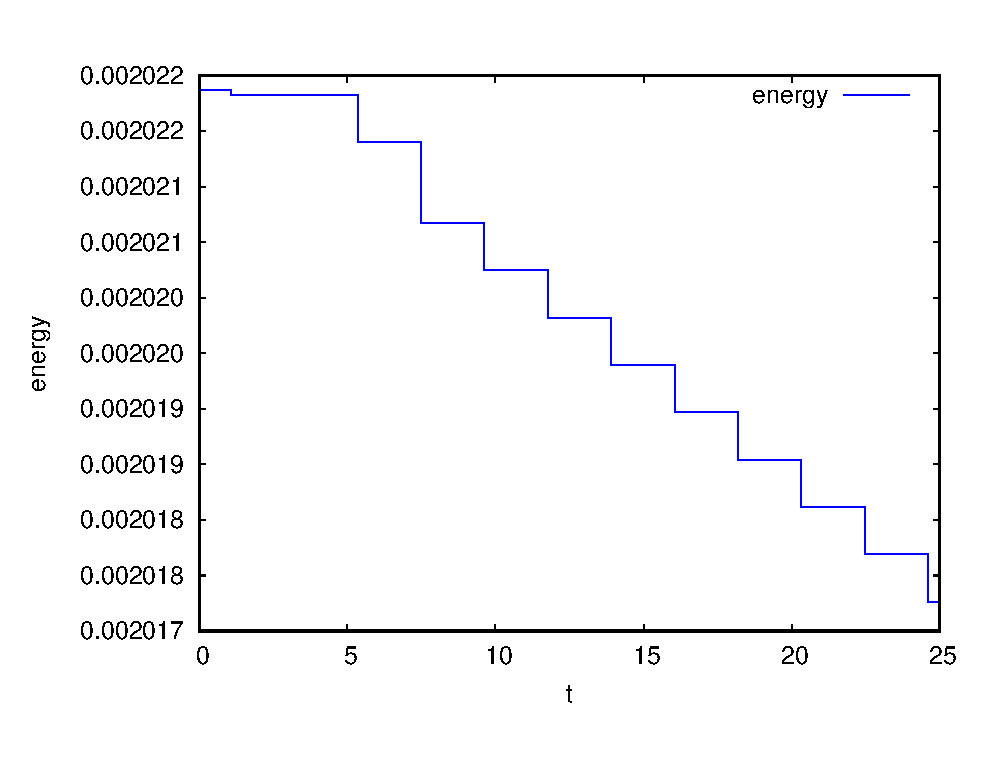
\includegraphics[scale=0.33]{content/pic/self_rot_25/kin_en.eps}
        \caption{Кинетическая энергия}
        \label{fig:self_rot_25_kin_en}
    }
    \hspace{10pt}
    \subf{0.3\textwidth}{
        \centering
        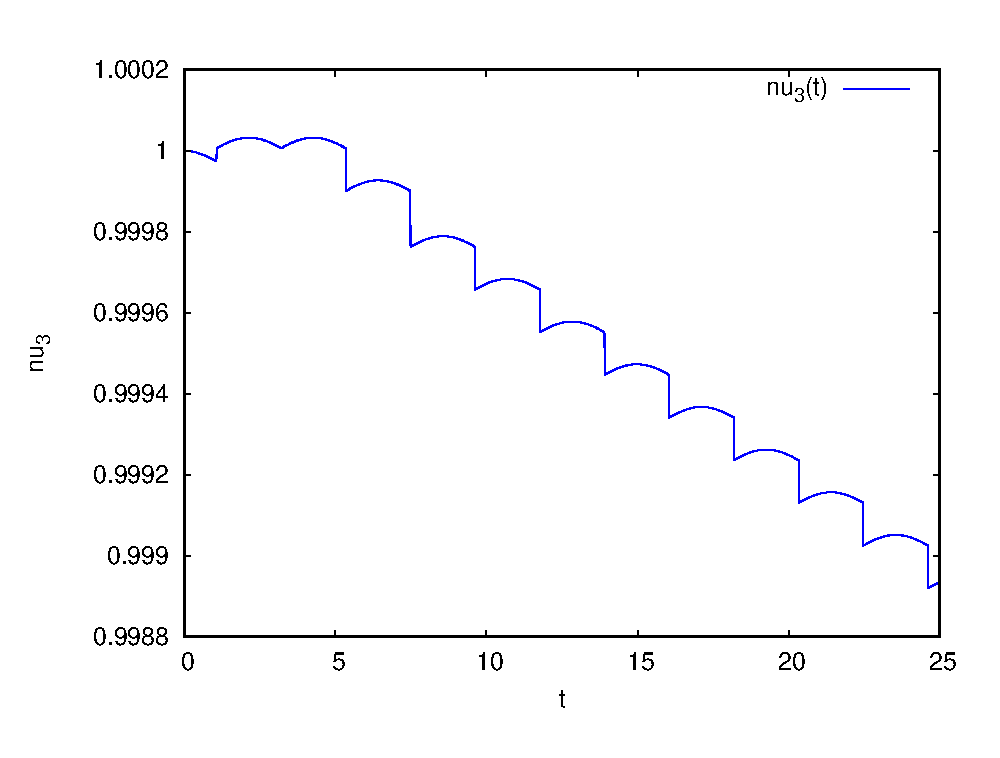
\includegraphics[scale=0.33]{content/pic/self_rot_25/nu3.eps}
        \caption{Угловая скорость экипажа}
        \label{fig:self_rot_25_nu3}
    }
    \hspace{10pt}
    \subf{0.3\textwidth}{
        \centering
        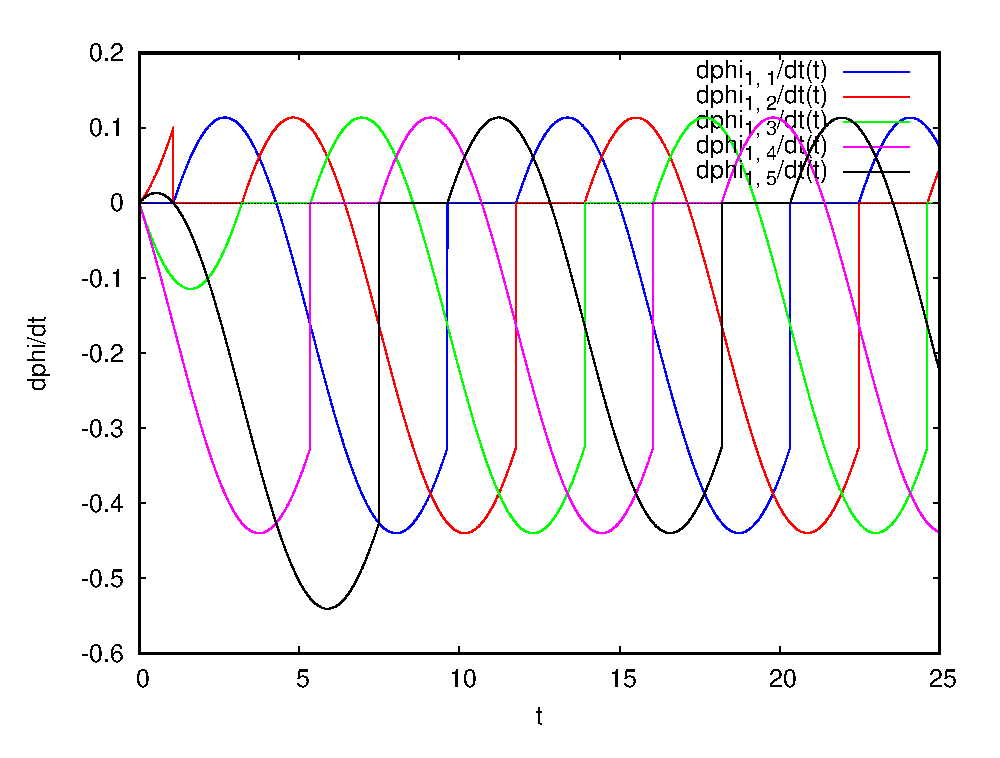
\includegraphics[scale=0.33]{content/pic/self_rot_25/rol_vel.eps}
        \caption{Угловые скорости роликов}
        \label{fig:self_rot_25_rol_vel}
    }
    \newline
    \subf{0.3\textwidth}{
        \centering
        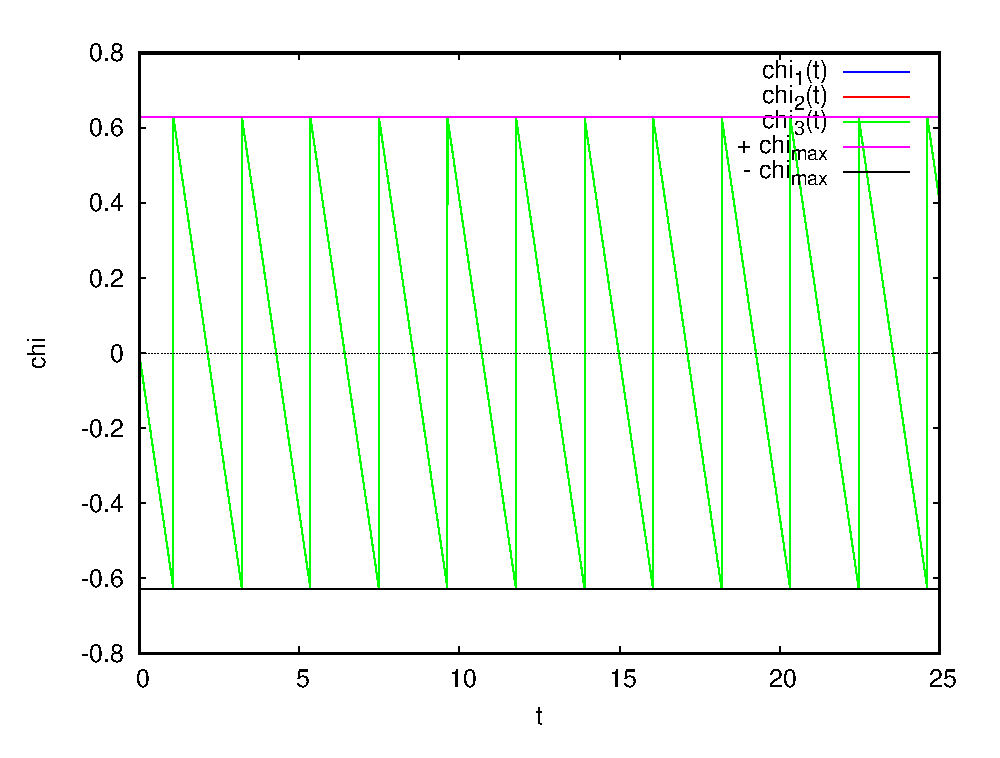
\includegraphics[scale=0.33]{content/pic/self_rot_25/chi.eps}
        \caption{Углы поворота колес}
        \label{fig:self_rot_25_chi}
    }
    \hspace{10pt}
    \subf{0.3\textwidth}{
        \centering
        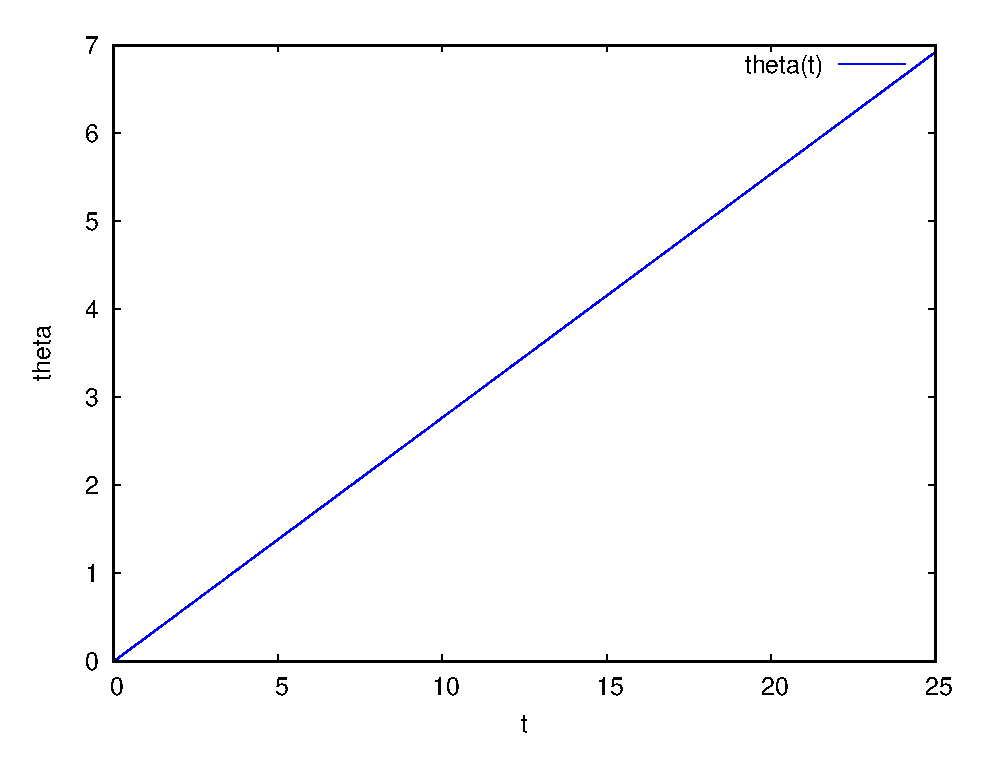
\includegraphics[scale=0.33]{content/pic/self_rot_25/theta.eps}
        \caption{Угол поворота экипажа}
        \label{fig:self_rot_25_theta}
    }
    \hspace{10pt}
    \subf{0.3\textwidth}{
        \centering
        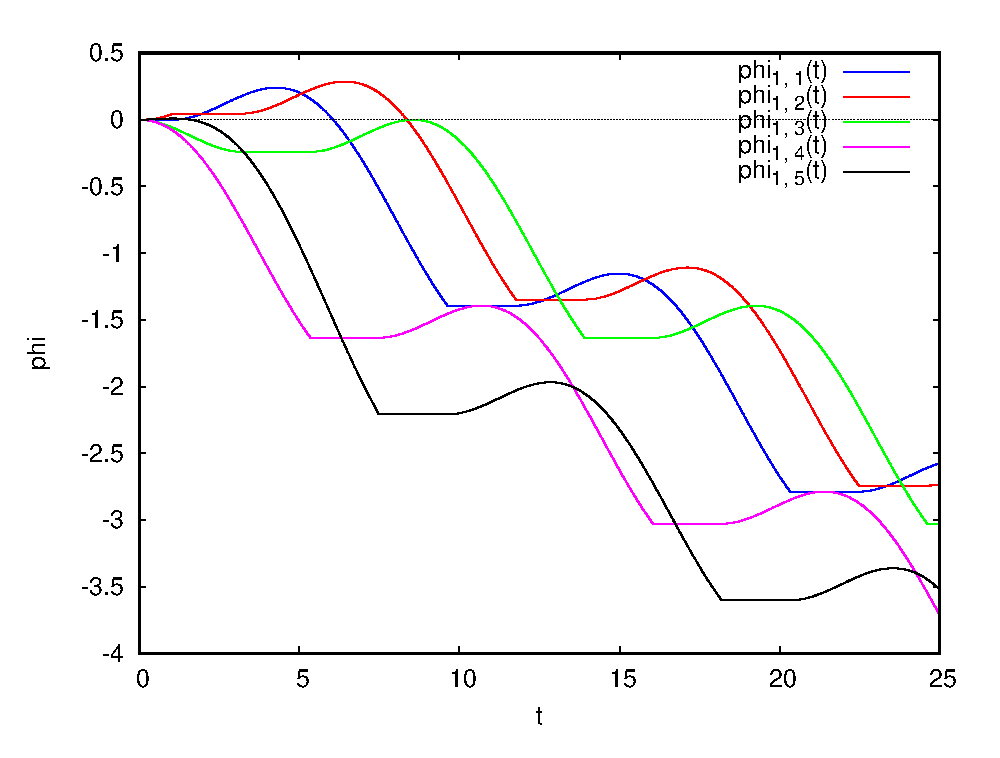
\includegraphics[scale=0.33]{content/pic/self_rot_25/rol_ang.eps}
        \caption{Углы поворота роликов}
        \label{fig:self_rot_25_rol_ang}
    }
    \caption{Вращение экипажа вокруг своей оси}
\end{figure}
\label{fig:self_rot}

\newpage

% \subsection{По прямой}

\begin{figure}[h]
    \hspace{-20pt}
    \subf{0.22\textwidth}{
        \centering
        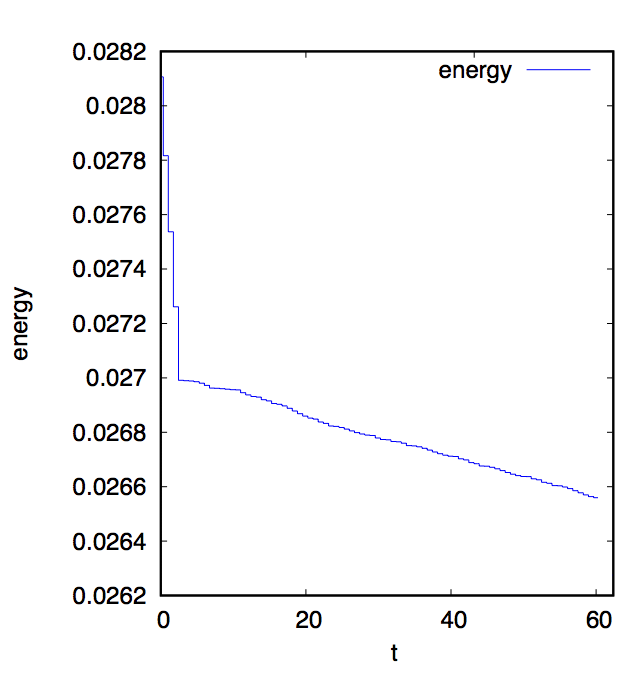
\includegraphics[scale=0.22]{content/pic/straight_60/kin_en.png}
        \caption{Кинетическая энергия}
        \label{fig:straight_60_kin_en}
    }
    \hspace{20pt}
    \subf{0.4\textwidth}{
        \centering
        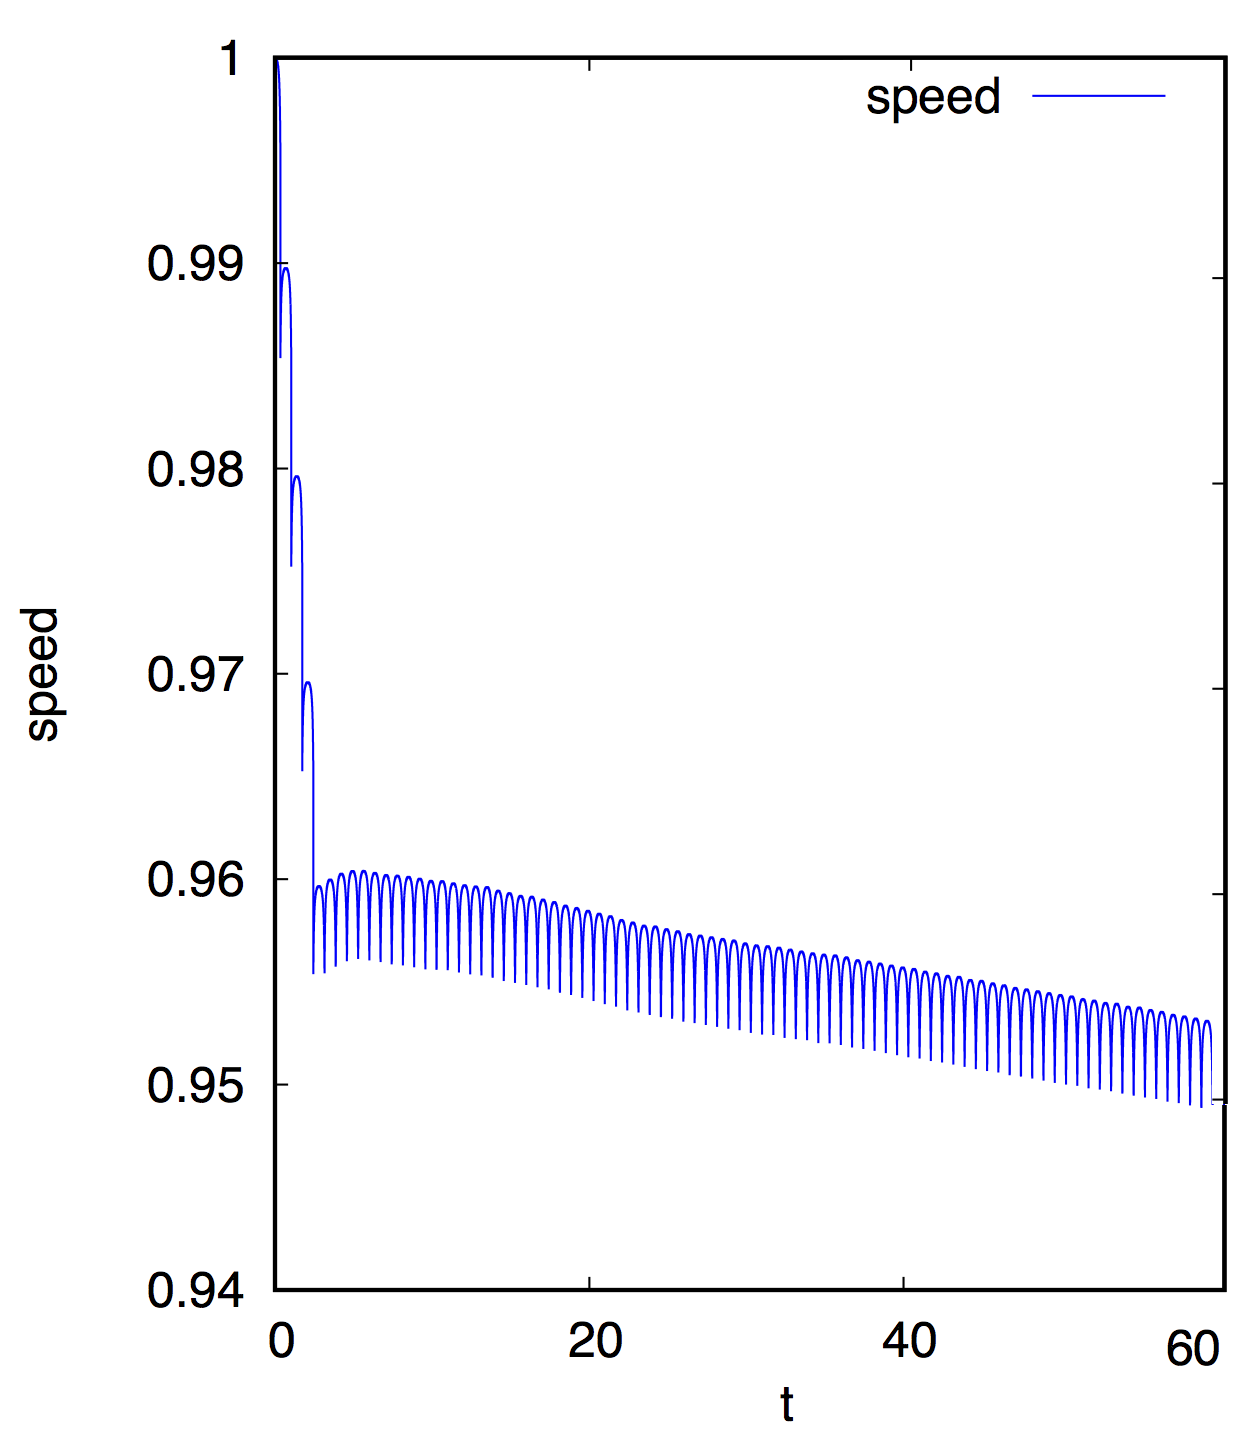
\includegraphics[scale=0.43]{content/pic/straight_60/v.png}
        \caption{Скорость центра масс}
        \label{fig:straight_60_v}
    }
    % \hspace{10pt}
    \subf{0.35\textwidth}{
        \centering
        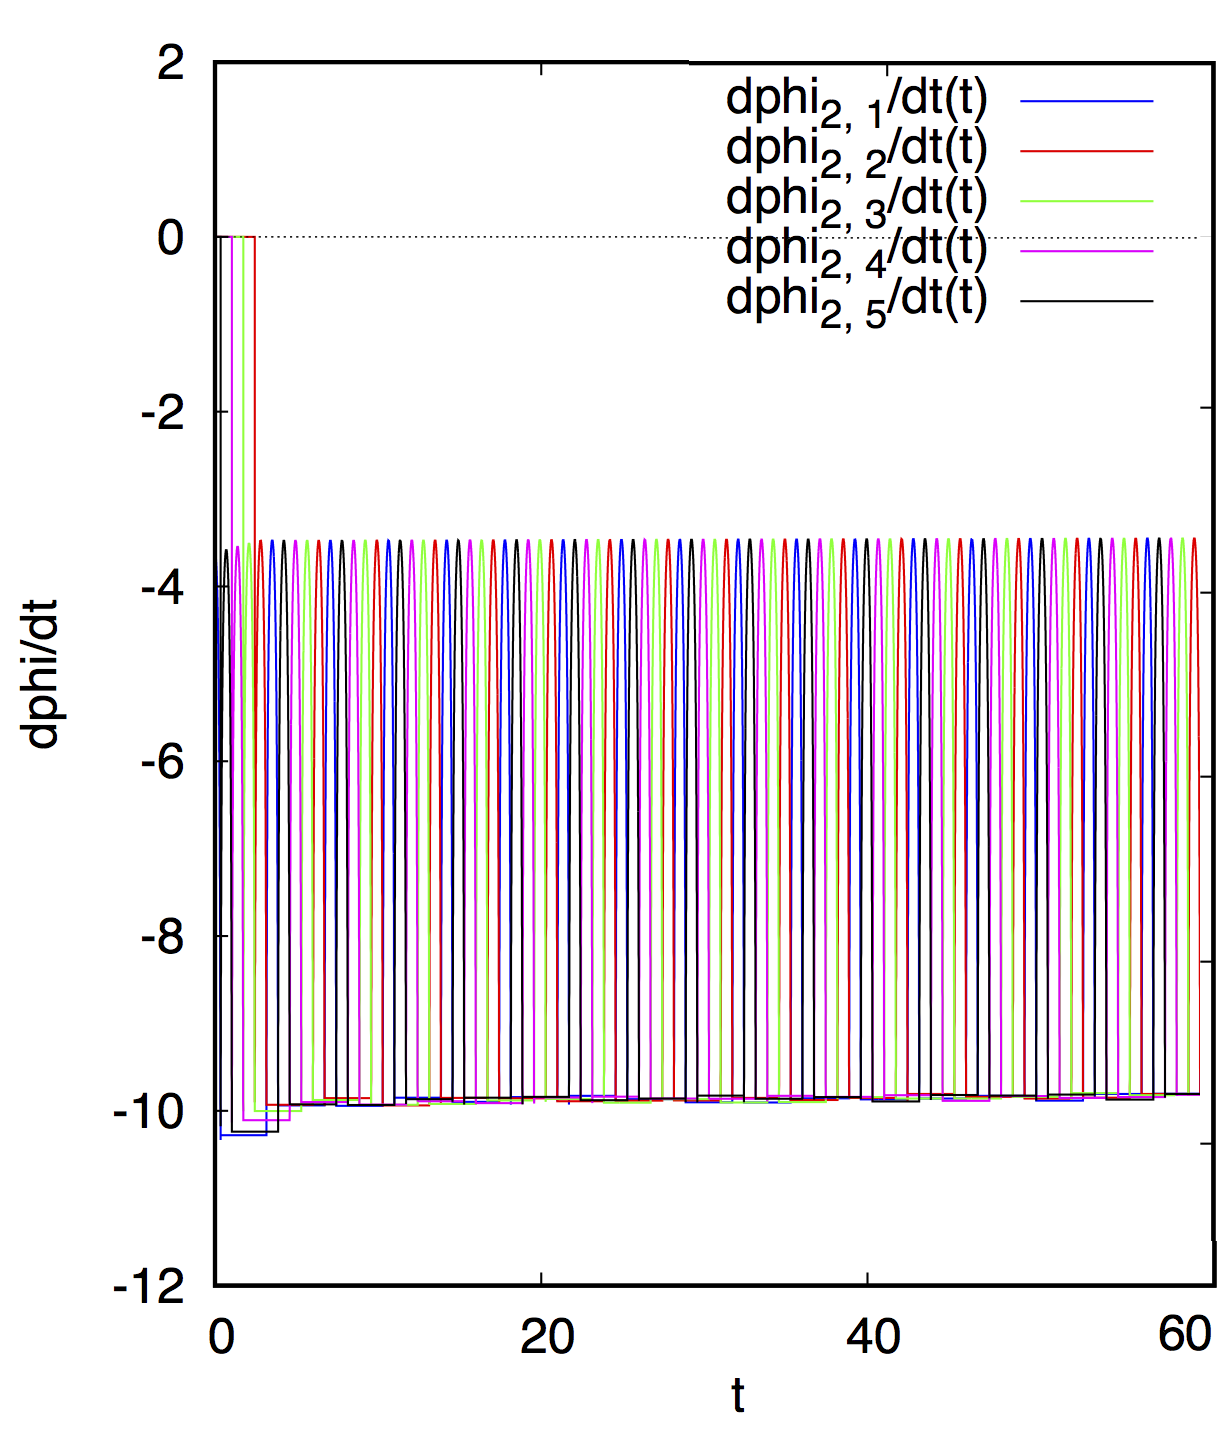
\includegraphics[scale=0.38]{content/pic/straight_60/nus2.png}
        \caption{Угловые скорости роликов на заднем колесе}
        \label{fig:straight_60_nus2}
    }
    \newline
    \subf{0.3\textwidth}{
        \centering
        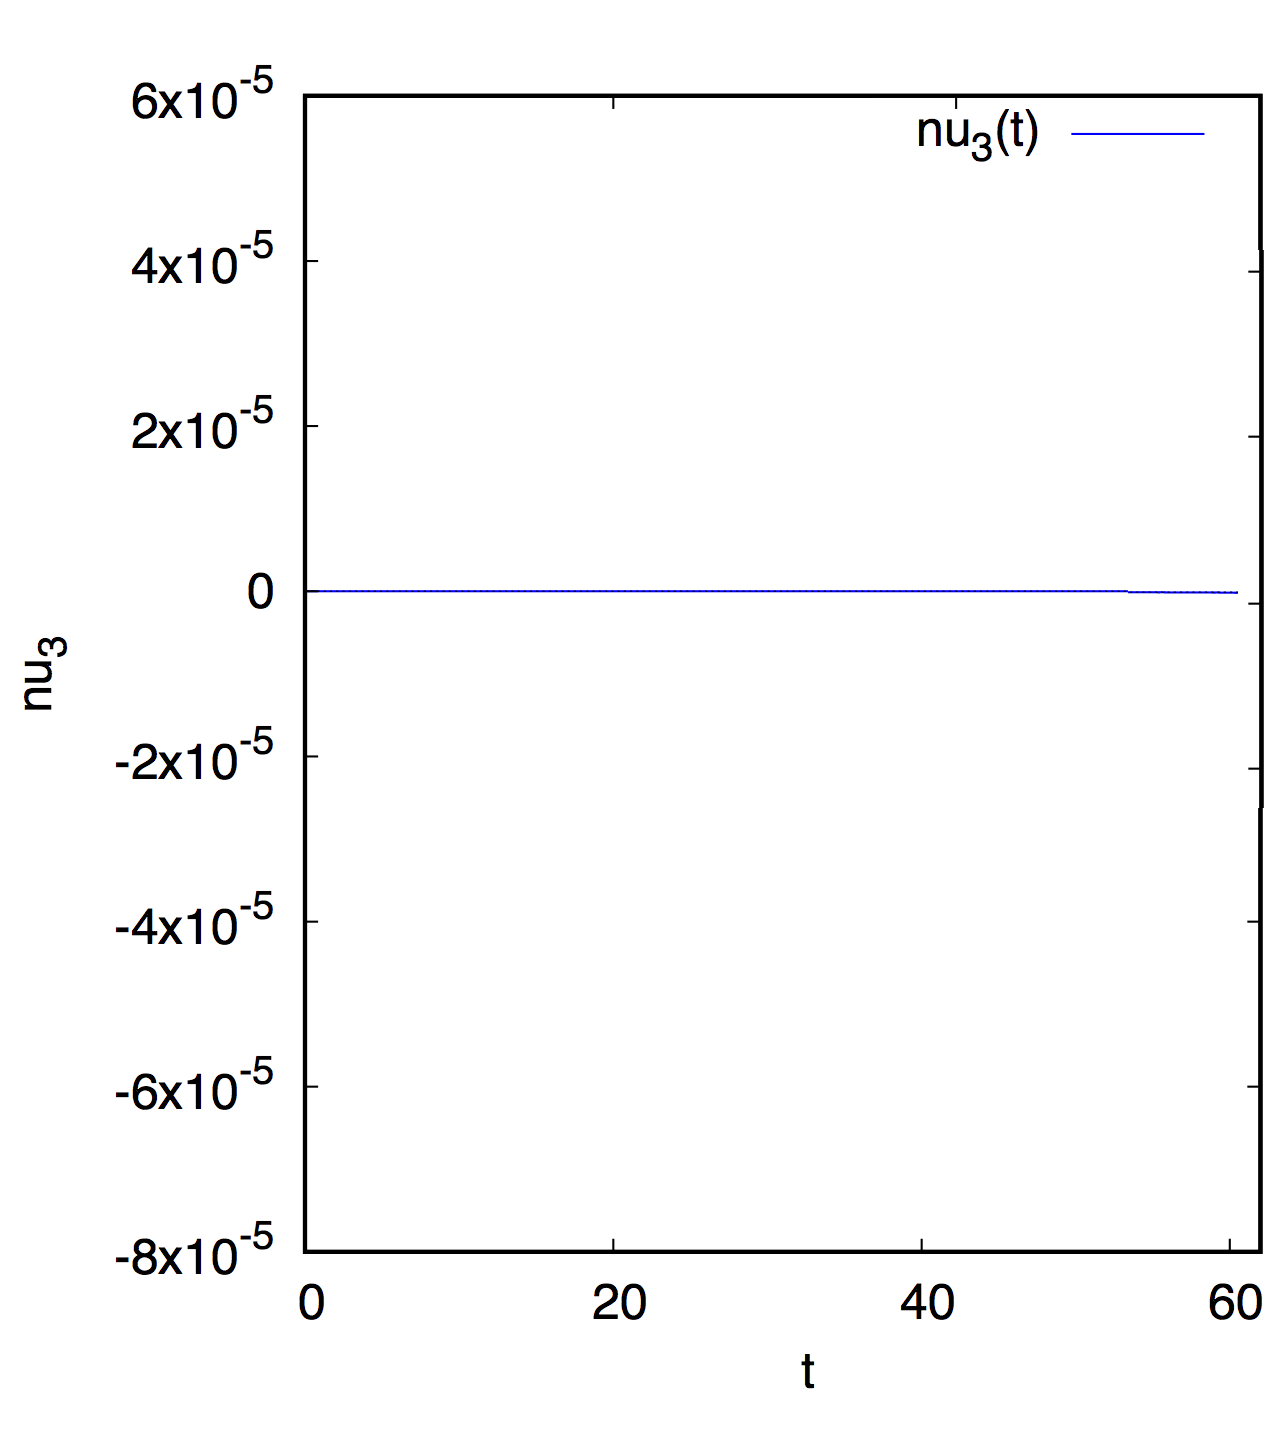
\includegraphics[scale=0.36]{content/pic/straight_60/nu3.png}
        \caption{Угловая скорость экипажа}
        \label{fig:straight_60_nu3}
    }
    \hspace{10pt}
    \subf{0.3\textwidth}{
        \centering
        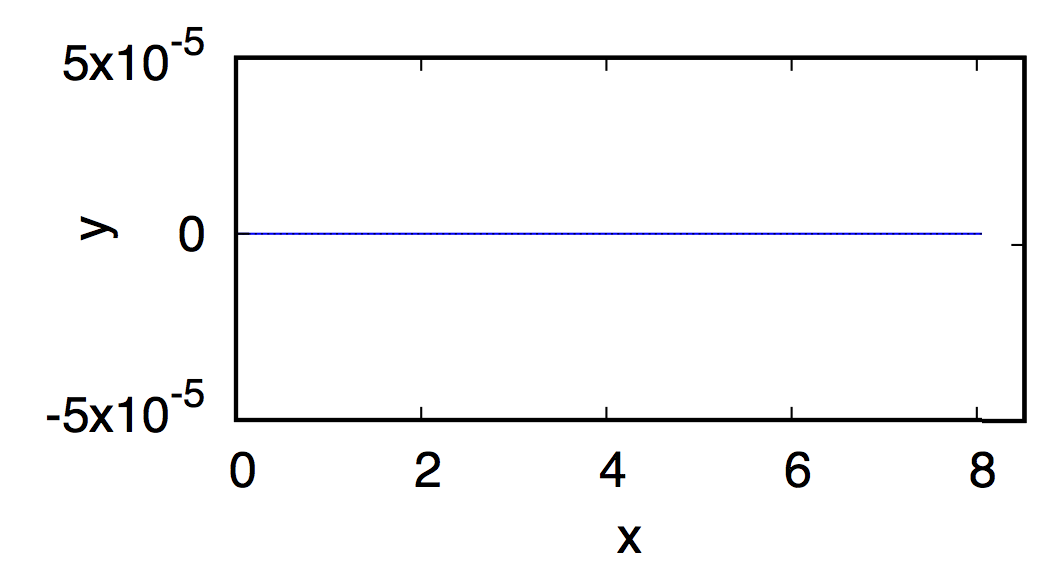
\includegraphics[scale=0.55]{content/pic/straight_60/traj.png}
        \caption{Траектория}
        \label{fig:straight_60_traj}
    }
    \hspace{10pt}
    \subf{0.3\textwidth}{
        \centering
        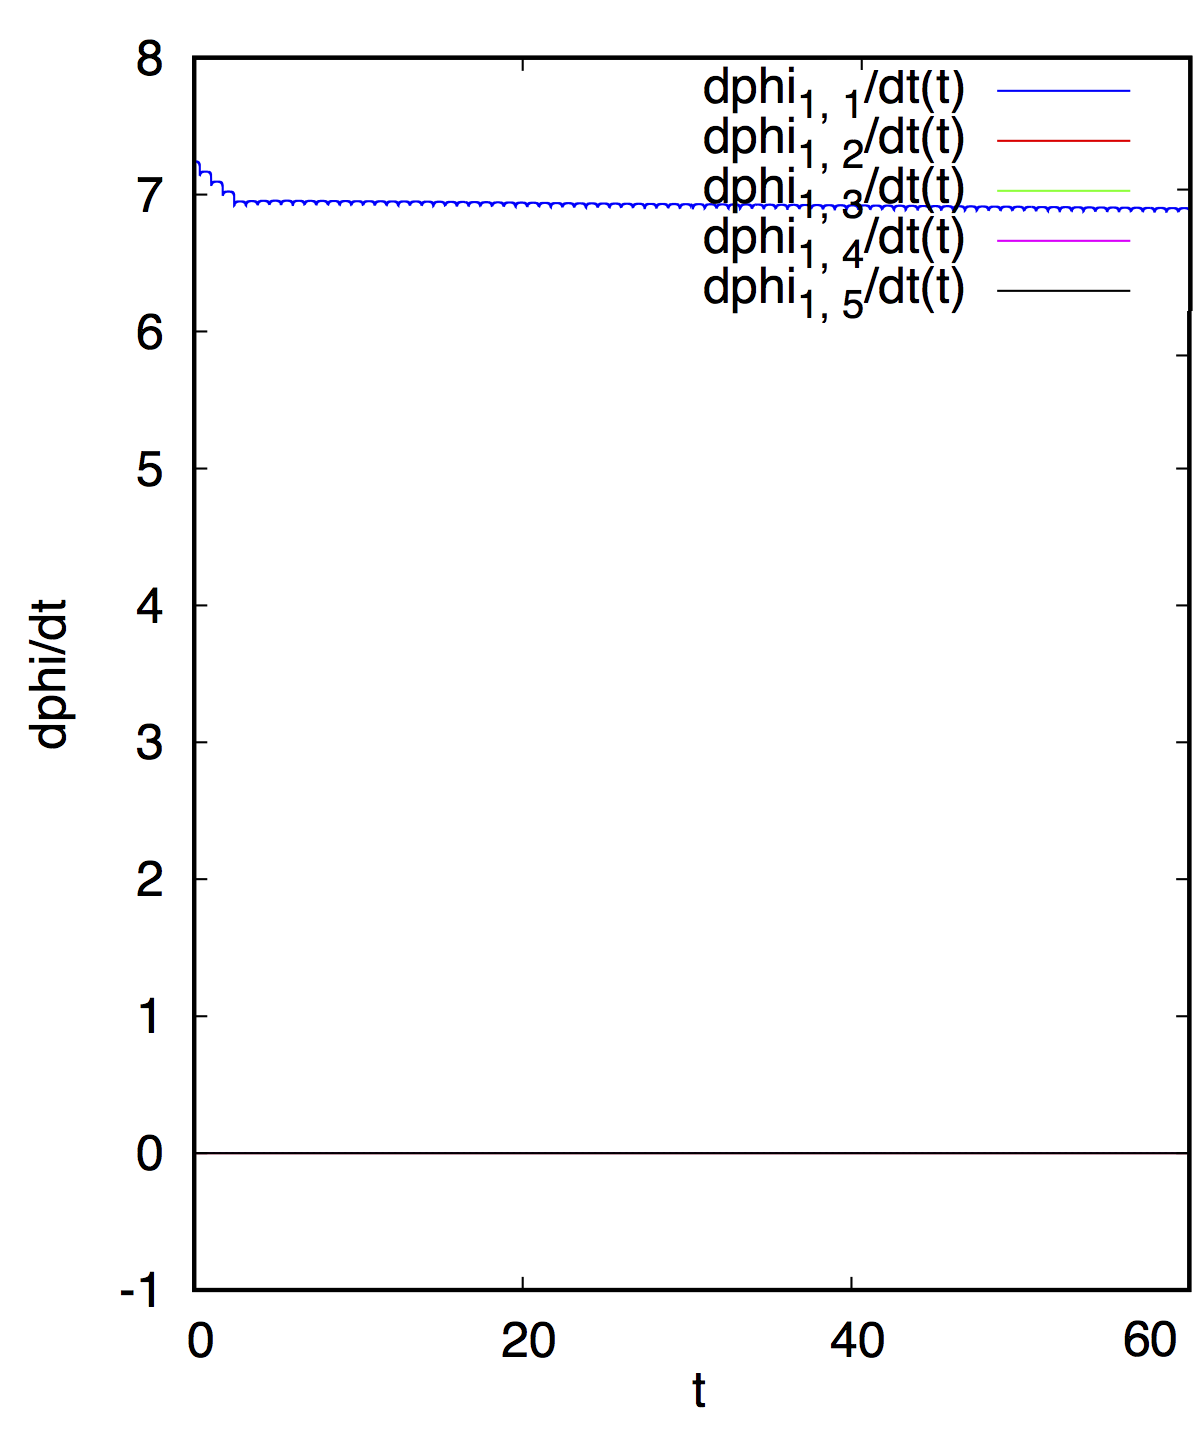
\includegraphics[scale=0.33]{content/pic/straight_60/nus1.png}
        \caption{Угловые скорости роликов на переднем колесе}
        \label{fig:straight_60_nus1}
    }
    \newline
    \subf{0.3\textwidth}{
        \centering
        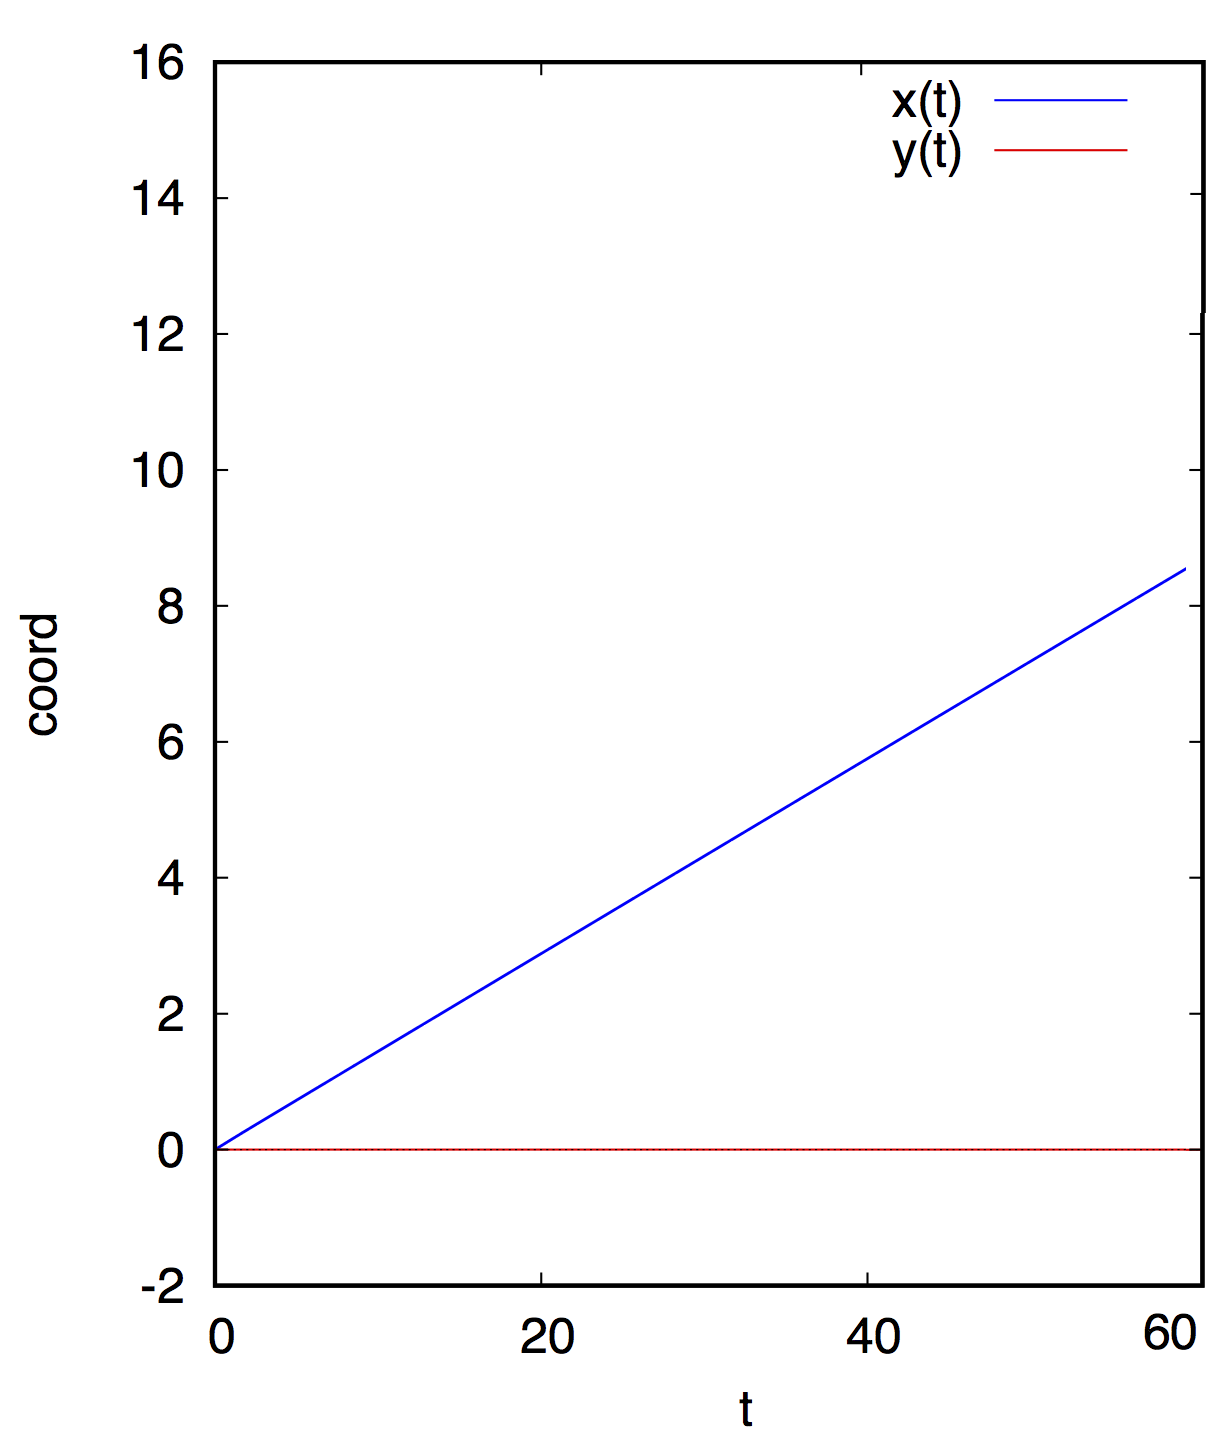
\includegraphics[scale=0.33]{content/pic/straight_60/xy.png}
        \caption{Координаты центра масс}
        \label{fig:straight_60_xy}
    }
    \hspace{10pt}
    \subf{0.3\textwidth}{
        \centering
        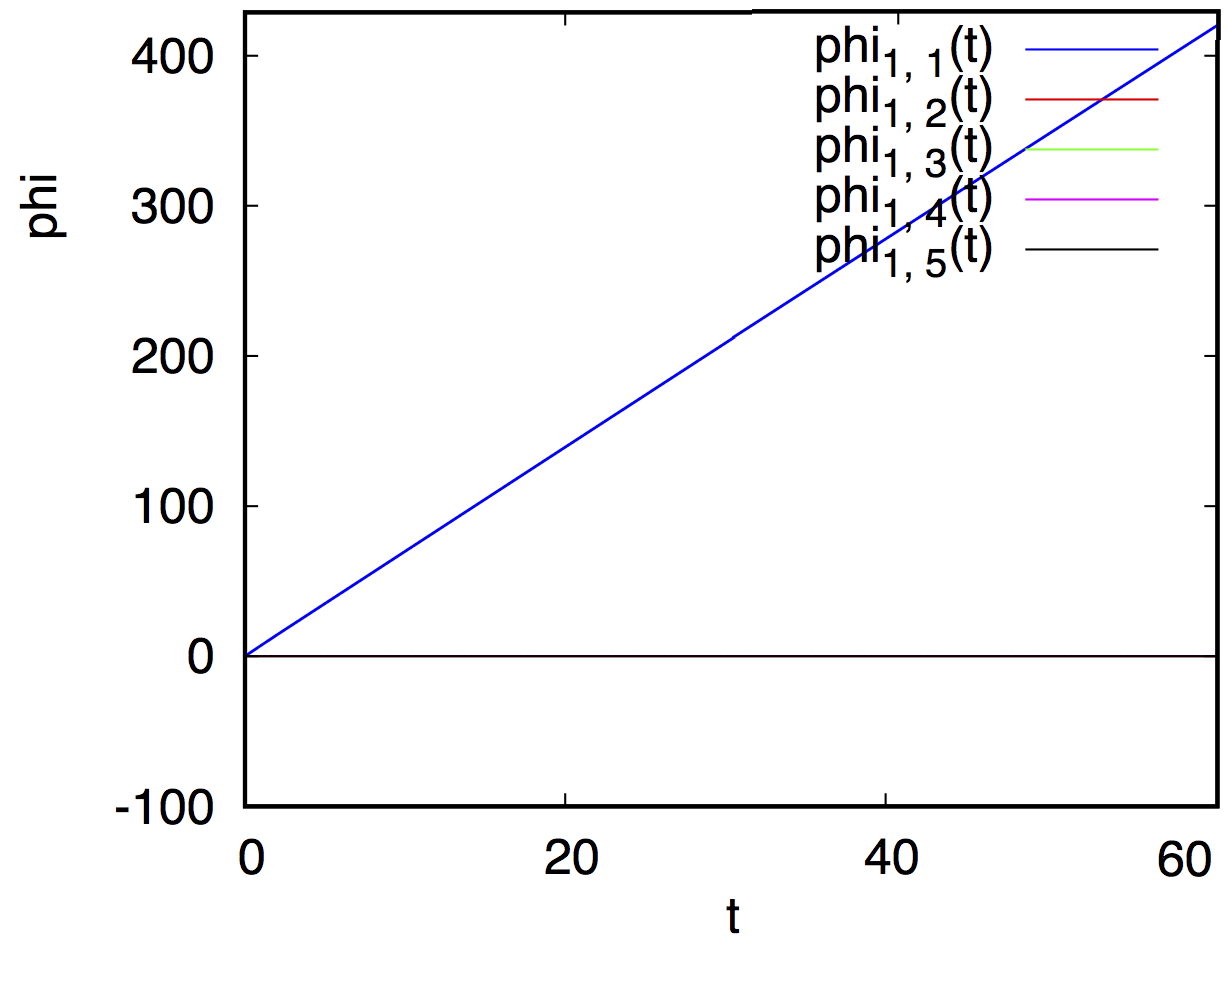
\includegraphics[scale=0.43]{content/pic/straight_60/phi1.png}
        \caption{Углы поворота роликов на переднем колесе}
        \label{fig:straight_60_phi1}
    }
    \hspace{10pt}
    \subf{0.3\textwidth}{
        \centering
        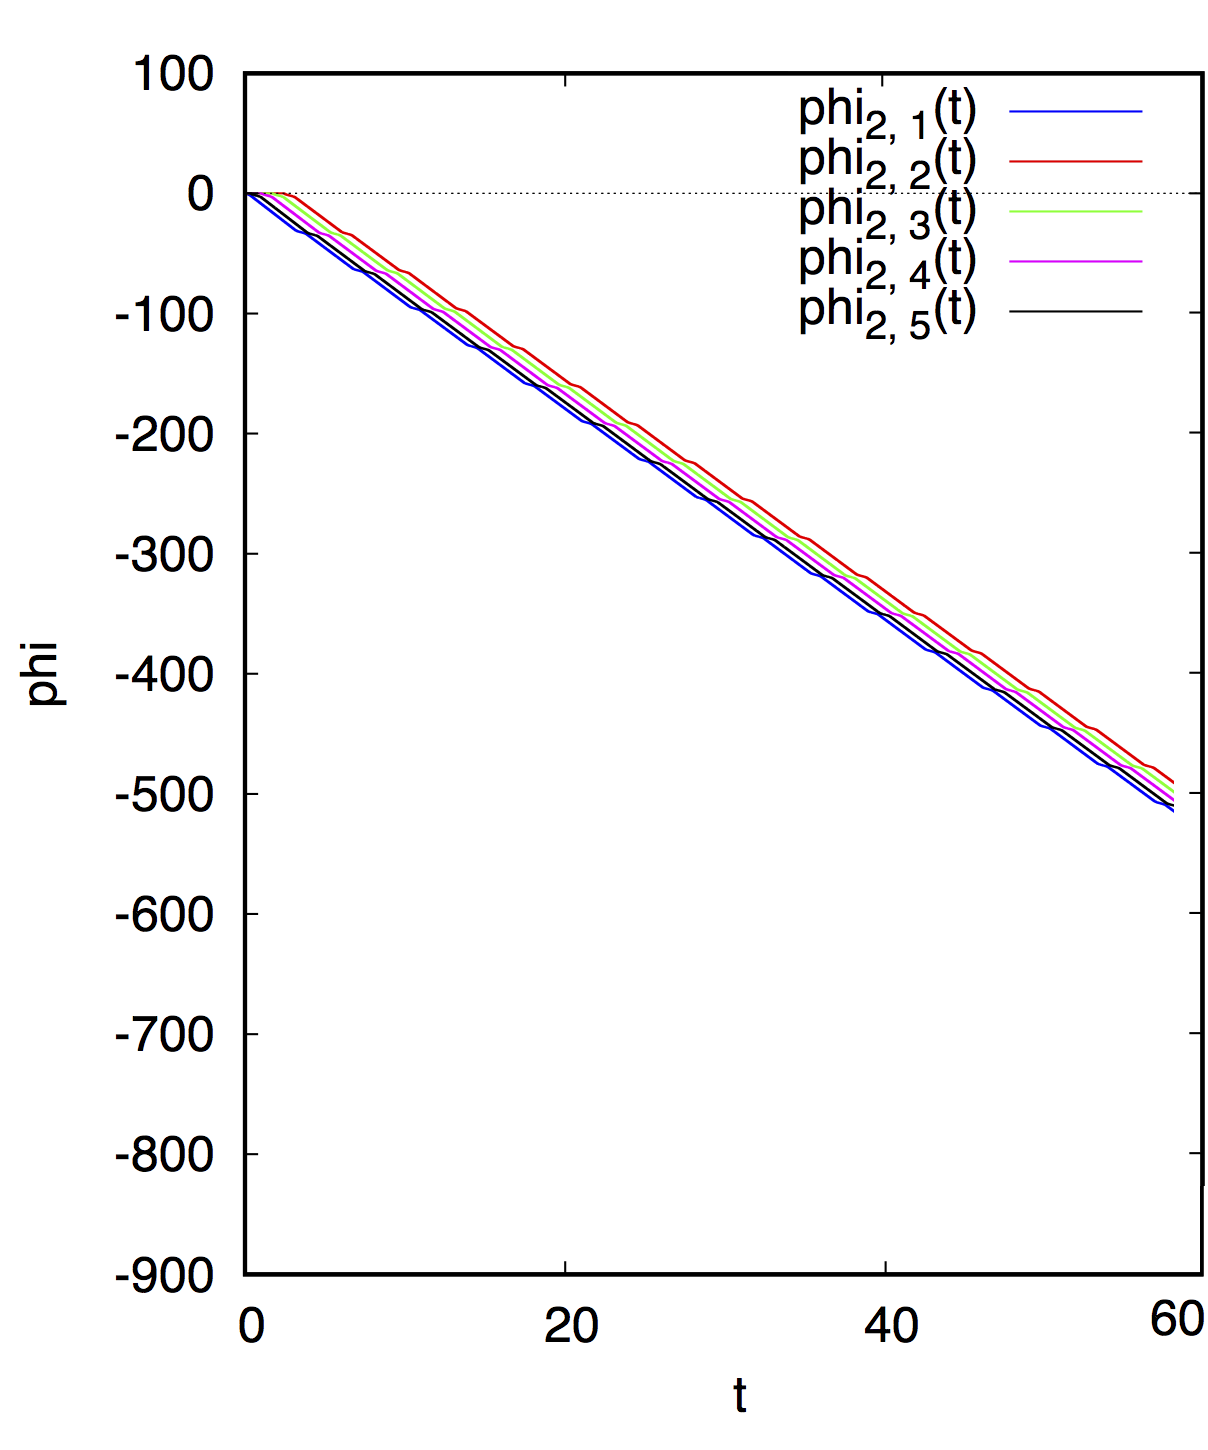
\includegraphics[scale=0.33]{content/pic/straight_60/phi2.png}
        \caption{Углы поворота роликов на заднем колесе}
        \label{fig:straight_60_phi2}
    }
    \caption{Движение экипажа по прямой}
\end{figure}
\label{fig:straight}

\newpage

% \subsection{С закруткой}

\begin{figure}[h]
    \subf{0.3\textwidth}{
        \centering
        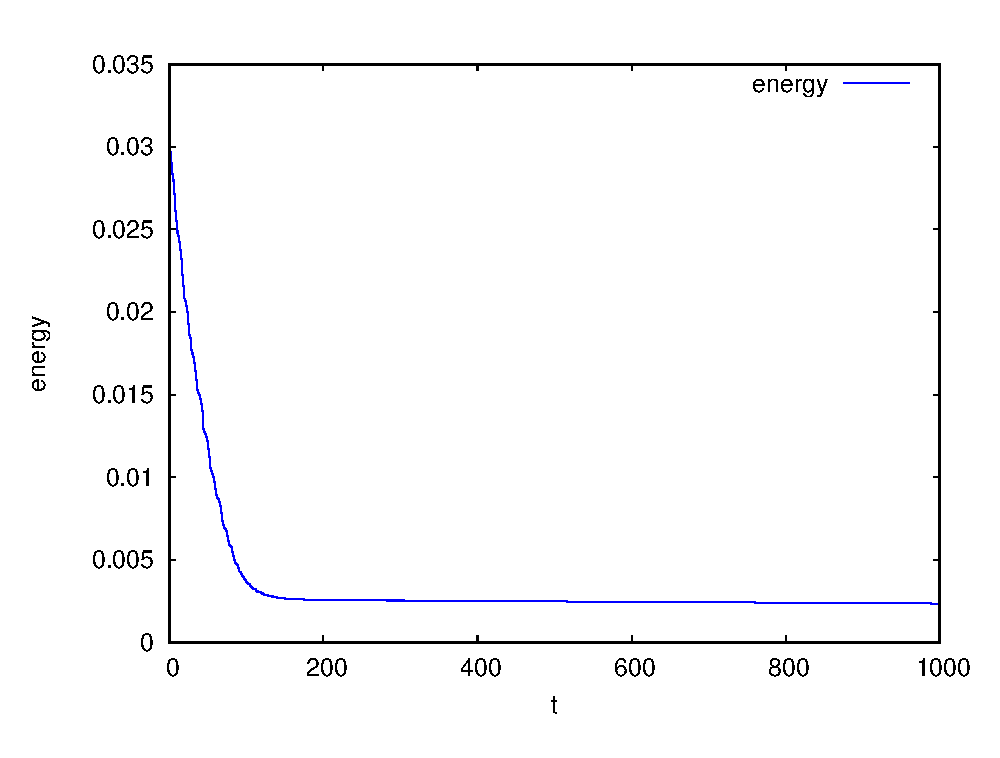
\includegraphics[scale=0.33]{content/pic/wrench_1000/kin_en.eps}
        \caption{Кинетическая энергия}
        \label{fig:wrench_1000_kin_en}
    }
    \hspace{10pt}
    \subf{0.3\textwidth}{
        \centering
        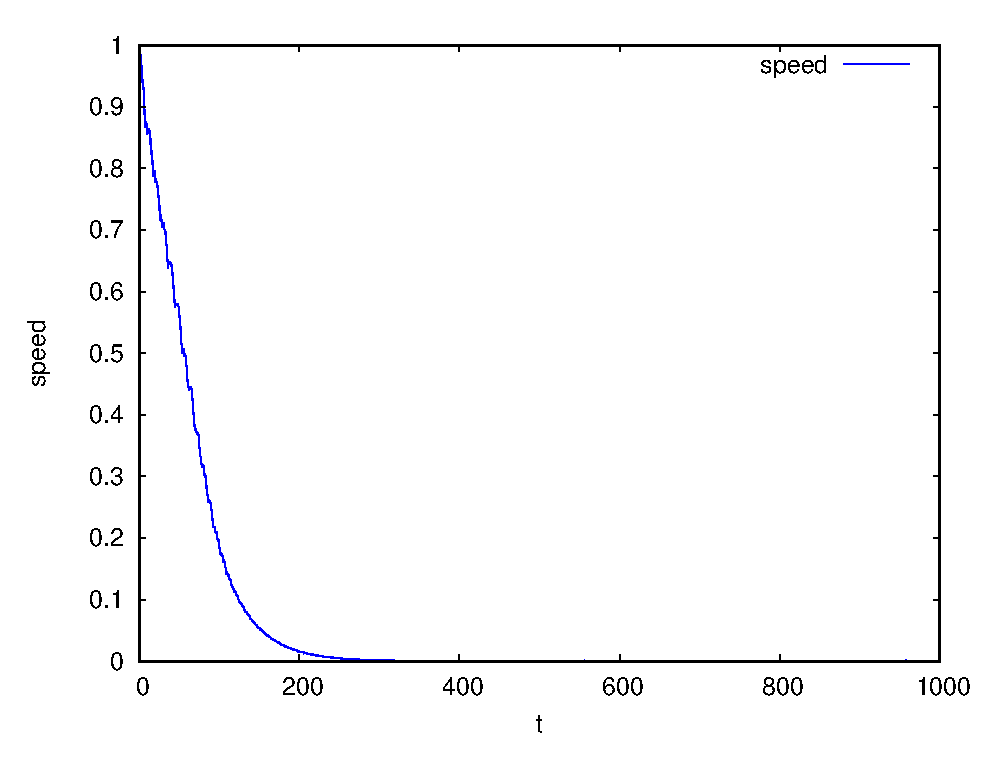
\includegraphics[scale=0.33]{content/pic/wrench_1000/v.eps}
        \caption{Скорость центра масс}
        \label{fig:wrench_1000_v}
    }
    \hspace{10pt}
    \subf{0.3\textwidth}{
        \centering
        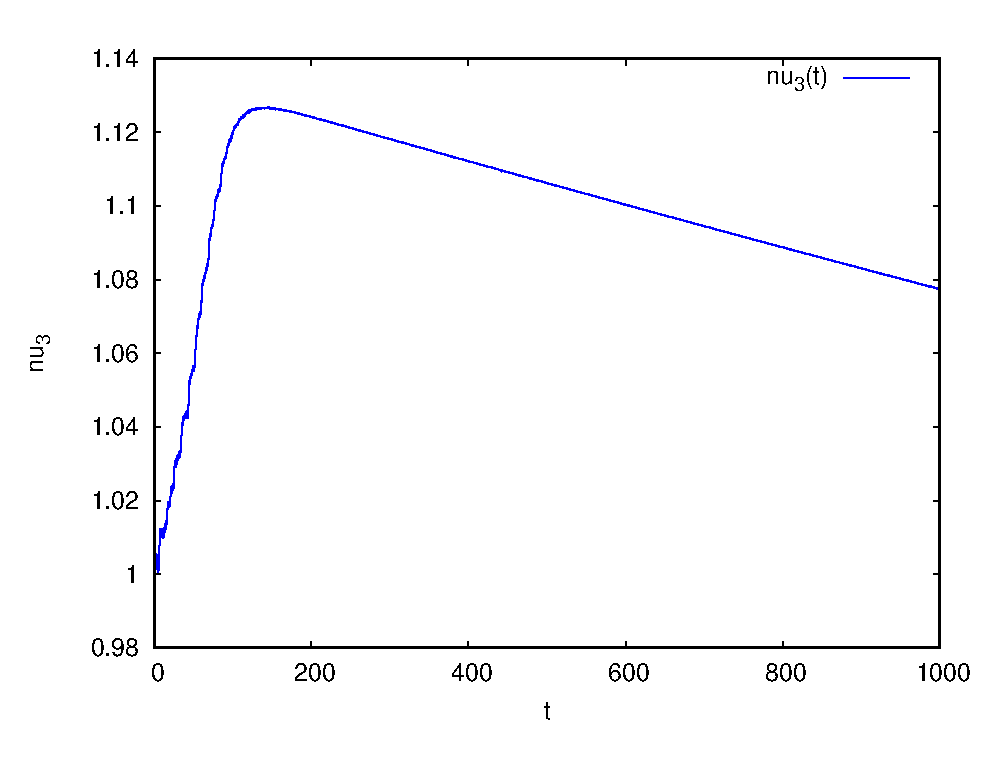
\includegraphics[scale=0.33]{content/pic/wrench_1000/nu3.eps}
        \caption{Угловая скорость экипажа}
        \label{fig:wrench_1000_nu3}
    }
    \newline
    \subf{0.45\textwidth}{
        \centering
        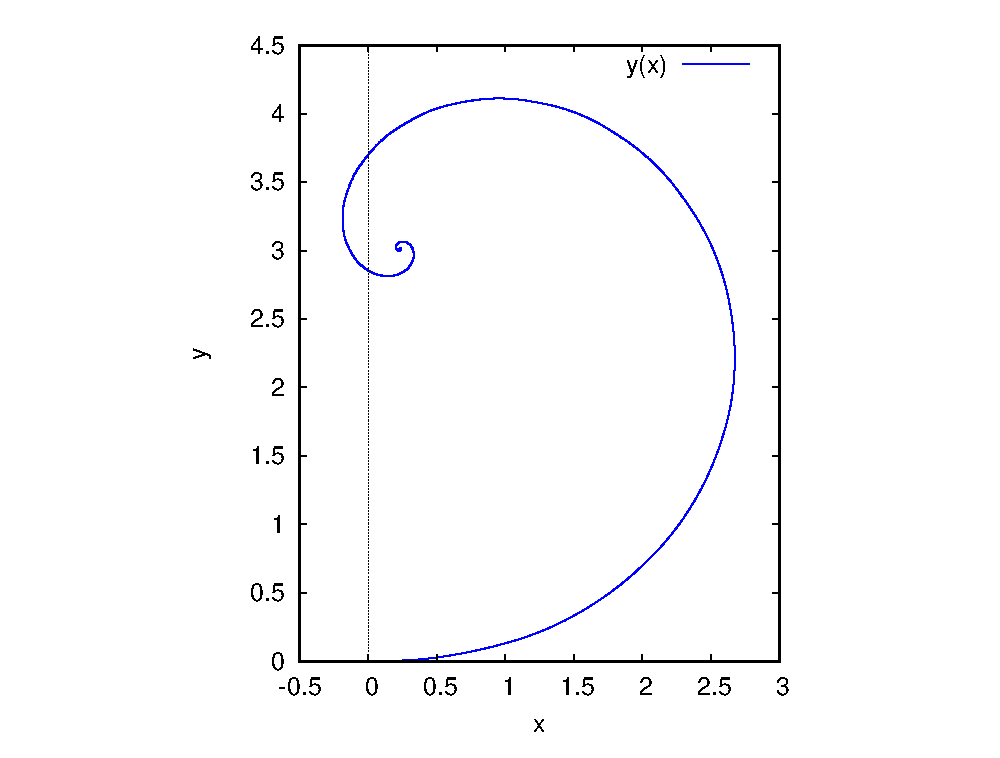
\includegraphics[scale=0.33]{content/pic/wrench_1000/traj.eps}
        \caption{Траектория центра масс}
        \label{fig:wrench_1000_traj}
    }
    \hspace{10pt}
    \subf{0.45\textwidth}{
        \centering
        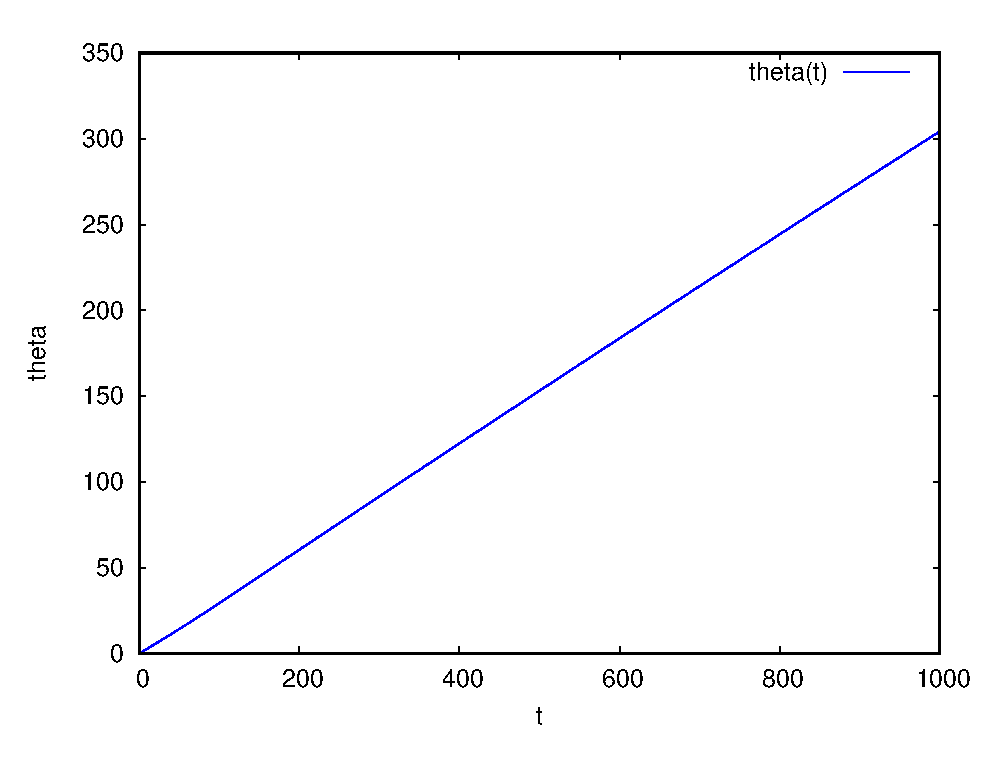
\includegraphics[scale=0.33]{content/pic/wrench_1000/theta.eps}
        \caption{Угол поворота экипажа}
        \label{fig:wrench_1000_theta}
    }
    \newline
    \subf{0.45\textwidth}{
        \centering
        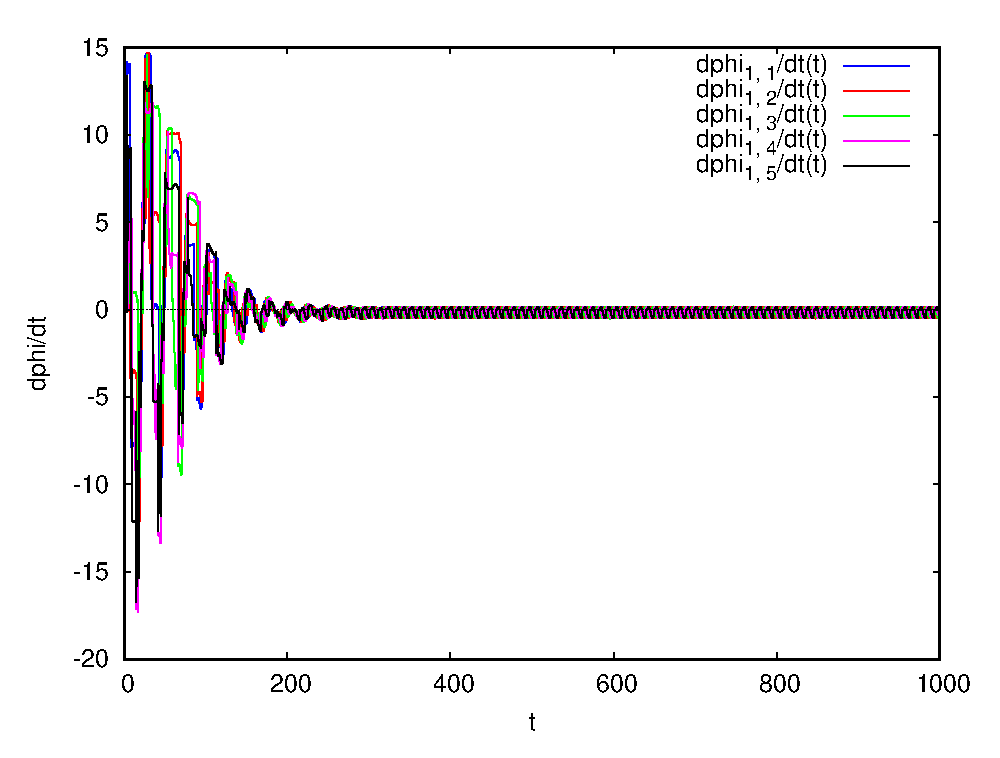
\includegraphics[scale=0.33]{content/pic/wrench_1000/nus1.eps}
        \caption{Угловые скорости роликов на переднем колесе}
        \label{fig:wrench_1000_nus1}
    }
    \hspace{10pt}
    \subf{0.45\textwidth}{
        \centering
        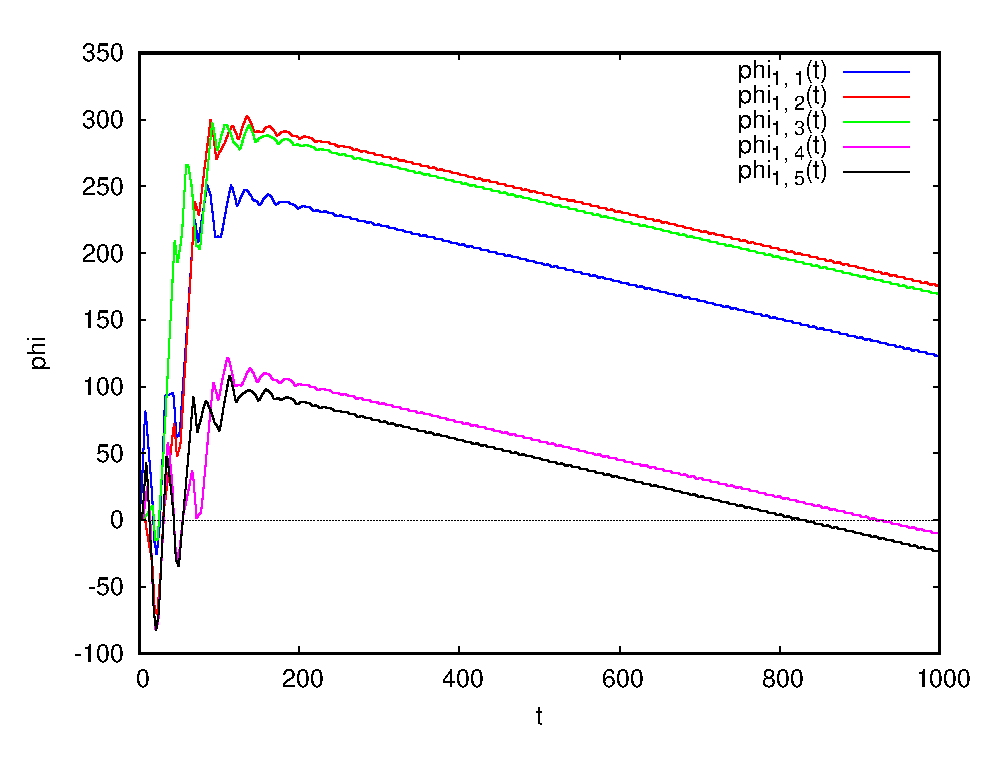
\includegraphics[scale=0.33]{content/pic/wrench_1000/phi1.eps}
        \caption{Углы поворота роликов на переднем колесе}
        \label{fig:wrench_1000_phi1}
    }
    \caption{Движение экипажа с закруткой}
\end{figure}
\label{fig:wrench}

\newpage